\documentclass[a4paper]{article}
\usepackage[UTF8]{ctex}
\usepackage{geometry}
\usepackage{graphicx}
\usepackage{url}
\usepackage{multirow}
\usepackage{array}
\usepackage{booktabs}
\usepackage{url}
\usepackage{enumitem}
\usepackage{graphicx}
\usepackage{float}
\usepackage{amssymb}
\usepackage{amsmath}
\usepackage{subfig}
\usepackage{longtable}
\usepackage{pifont}
\usepackage{color}

\allowdisplaybreaks

\geometry{a4paper, scale=0.78}

% \begin{figure}[H]
%     \centering
%     \includegraphics[width=.55\textwidth]{E.png}
%     \caption{矩阵与列向量的乘法}
%     \label{fig:my_label_1}
% \end{figure}

% \left\{
% \begin{array}{ll}
%       x+2x+z=2 & \\
%       3x+8y+z=12 & \\
%       4y+z=2
% \end{array}
% \right.

% \begin{enumerate}[itemindent = 1em, itemsep = 0.4pt, parsep=0.5pt, topsep = 0.5pt]

% \end{enumerate}

%\stackrel{a}{\longrightarrow}

%\underbrace{}_{} %下括号

%\tableofcontents %目录,并且目录页不记录页码
% \tableofcontents
% \newpage
% \setcounter{page}{1} %new page
% \clearpage

\title{Restricted Boltzmann Machine}
\author{Chen Gong}
\date{28 February 2020}

\begin{document}
\maketitle
%\pagestyle{empty}
\tableofcontents
\newpage
%\pagestyle{fancy}
\setcounter{page}{1} %new page
\clearpage

\section{Background}
本小节主要介绍的是受限玻尔兹曼机(Restricted Boltzmann Machine, RBM)。本小节,我们主要讨论的是什么是Boltzmann Machine,然后讲讲它的历史,为我们引出Restricted Boltzmann Machine做铺垫。
\subsection{什么是Boltzmann Machine?}
其实Boltzmann Machine就是一种Markov Random Field,也就是无向图而已。那么,Boltzmann Machine和普通的无向图有什么不同呢?区别就在于\textbf{Markov Random Field with hidden nodes},即为无向图中的节点,有一部分是可观测的,一部分是不可观测的。

马尔可夫随机场中的每一个节点代表一个随机变量(Random variable),而所有的Random variable可以被分为两类,即为observed variable $v$和hidden variable $h$;如下图所示,灰色代表不可观测变量,白色代表可观测变量。
\begin{figure}[H]
    \centering
    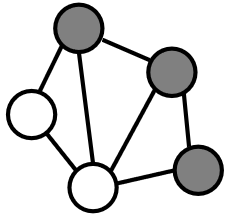
\includegraphics[width=.25\textwidth]{微信图片_20200228220817.png}
    \caption{玻尔兹曼机实例图}
    
\end{figure}

\subsection{无向图中的因子分解}
在无向图中,最重要的就是因子分解,\textbf{因子分解是对联合概率进行建模}。它基于最大团的概念来进行分解的,理论基础是Hammersley Clifford Theorem。因子分解的公式表达为:
\begin{equation}
    P(X) = \frac{1}{Z} \prod_{i=1}^k \phi_i (x_{c_i})
\end{equation}
其中,$x_{c_i}$表示第$i$个最大团;$x_{c_i}$表示第$i$个最大团中的随机变量组成的集合;$\phi_i (x_{c_i})$表示他们的势函数(Potential Function)。而$Z$是归一化因子,有时也被称为配分函数(Partition Function)。注意两个约束条件,1. $\phi_i (x_{c_i})$是严格正定的;2. $Z$是归一化因子:
$$
Z = \sum_X \prod_{i=1}^k \phi_i (x_{c_i}) = \sum_{x_1}\sum_{x_2}\cdots \sum_{x_p} \prod_{i=1}^k \phi_i (x_{c_i})
$$
在概率图模型中,没有特殊情况都是指离散变量。

因为\textbf{指数族分布是满足最大熵原理的分布}(个人觉得这个最大熵原理简直无处不在,也是为什么很多函数,动不动就变指数函数的原因,实际上是有理论依据的,不是随便加的)。为了简化表达,我们令:
$$
\phi_i (x_{c_i}) = \exp \left\{ -\mathrm{E}(x_{c_i}) \right\}
$$
而且这样就正好满足了$\phi_i (x_{c_i})$是严格正定的需求,而E则被称为能量函数(Energy Function)。所以,联合概率分布,被改写为:
\begin{equation}
    P(X) = \frac{1}{Z} \prod_{i=1}^k \phi_i (x_{c_i}) = \frac{1}{Z} \exp\left\{ -\sum_{i=1}^k \mathrm{E}(x_{c_i}) \right\}
\end{equation}

而最大团中的所有变量,可以用$X$来表达,最后可以化简为一个和$X$相关的能量函数,表达为:
\begin{equation}
    P(X) = \frac{1}{Z} \exp (-\mathrm{E}(X))
\end{equation}
很显然,这个分布符合指数族分布的形式,被我们称为Boltzmann Distribution,或者Gibbs Distribution。所以,\textbf{如果取势函数是一个指数函数,那么整体为Boltzmann Distribution}。

前面讲了那么多,我们看了很多概念,我相信大家基本没搞懂,为什么叫“势函数”和“能量函数”,这种奇奇怪怪的叫法。下面我们来看看Boltzmann Distribution的历史,来帮助我们进行理解。

\subsection{Boltzmann Distribution的历史}
Boltzmann Distribution最早来自于统计物理学,这是一个物理学的概率,这里我们采用感性的理解方式。

一个物理系统由各种各样的粒子组成。而一个系统的状态(State),由其中各种各样的粒子的状态联合而成。系统状态的概率满足:
\begin{equation}
    P(\mathrm{State}) \propto \exp \left\{ -\frac{\mathrm{E}}{\mathrm{kT}} \right\}
\end{equation}
其中,$\mathrm{E}$为能量函数,$\mathrm{T}$表示温度,$\mathrm{k}$为一个系数。而能量函数是一个离散的分布,一个System可能有$M$个状态,每个状态对应一个值,如下所示:
\begin{table}[H]
    \centering
    \begin{tabular}{l|llllll}
         State & 1& 2& $\cdots$&i & $\cdots$ & M \\
         \hline
        P   & $p_1$& $p_2$& $\cdots$ & $p_i$ & $\cdots$ & $p_M$ \\
    \end{tabular}
    \label{tab:my_label}
\end{table}

因为粒子有速度,受到其他粒子的干扰,所以$\mathrm{E}$和所有的粒子有关。对于$X$的概率函数,和$\mathrm{E}$成反比,能量越大,越不稳定,越容易发生状态的跃迁,当前状态出现的可能性就越小,概率就越低。

所以,如果没有外界的干扰,系统最终就到达一个能量比较低的稳态,因为能量高的状态都待不住。举一个例子,一个人年轻的时候,能量很强,很不稳定,工作对象什么的都很容易换。到了中年以后,这个时候可能追求的是自己的事业上的成功,而相对稳定了一些。到了老年,见的实在是太多了,这是追求的是一种心灵上的平静,内心基本没有什么冲动,一切回归平稳。

这就是无向图中一些概念的来源,用来辅助理解。这里我谈谈自己的理解:一个无向图就是一个系统,系统包括所有的节点,所以系统的状态就是系统中所有节点的联合概率。这个系统的状态的概率和内部的每一个节点都有关系,我们可以用能量函数来进行衡量一个状态出现的可能性,而能量越高的状态越容易发生转移,出现的概率越低,反之亦然。

\subsection{小结}
本节主要描述了,什么是Boltzmann Machine,核心就是节点分为可观测和不可观测的马尔可夫随机场。并且,概率图的联合分布,当势函数为指数函数时,联合分布是玻尔兹曼分布(吉布斯分布)。随后我们介绍了Boltzmann分布在统计物理学中的来源,来辅助我们对无向图中的一些概念的理解。介绍完了Boltzmann Machine,下面将引出Restricted Boltzmann Machine。

\section{Restricted Boltzmann Machine模型表示}
Boltzmann Machine就是内部的所有节点分为可观测和不可观测的马尔可夫随机场。假设一共有$p$个节点,$m$个不可观测的节点组成集合$h$,$n$个可观测的节点组成集合$v$。即为:
\begin{equation}
    X = \begin{bmatrix}
    x_1 \\
    x_2 \\
    \vdots \\
    x_p
    \end{bmatrix}
    = 
    \begin{bmatrix}
    h \\
    v
    \end{bmatrix}
    ,\quad
    h = 
    \begin{bmatrix}
    h_1 \\
    h_2\\
    \vdots \\
    h_m
    \end{bmatrix}
    ,\quad
    v = 
    \begin{bmatrix}
    v_1 \\
    v_2\\
    \vdots \\
    v_n
    \end{bmatrix}
\end{equation}
其中,$m+n=p$。Boltzmann Machine看着好像很好,但是实际上有一些问题。首先,Inference问题很难做,精确推断根本不可能,而近似推断基本也是intractable。正是因为有了这些问题,我们才要想办法对模型进行简化,从而得到了Restricted Boltzmann Machine。

\subsection{Restricted Boltzmann Machine}
我们只考虑Boltzmann Machine中,$h$和$v$之间的连接,不考虑它们内部的连接。如下图所示:
\begin{figure}[H]
    \centering
    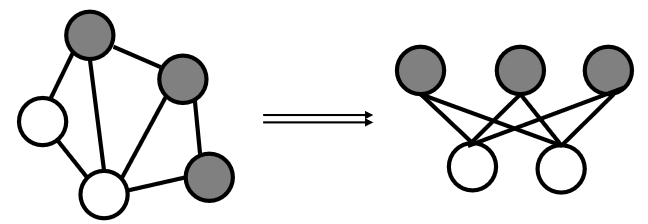
\includegraphics[width=.6\textwidth]{微信图片_20200229000824.png}
    \caption{玻尔兹曼机到受限玻尔兹曼机}
    \label{fig:my_label_1}
\end{figure}

我们接下来来定义能量函数的结构:
\begin{equation}
    \begin{split}
        P(X) 
        = & \frac{1}{Z} \exp (-\mathrm{E}(X)) \\
        P(v,h) 
        = &  \frac{1}{Z} \exp (-\mathrm{E}(v,h)) \\
    \end{split}
\end{equation}

接下来的问题就是如何定义$\mathrm{E}(v,h)$。考虑到,能量函数和系统内部的每一个节点之间有关系。由于不考虑节点内部之间的关系,所以能量函数可以被分解为:$h$节点中每个节点自身的影响,$v$节点中每个节点自身的影响,和$h$和$v$节点之间的影响。前两者考虑的是点自身的影响,后者是考虑两个集合中的点连接的边的影响。

下一步则假设,两个集合中的点连接的边的关系用矩阵$x=[w_{ij}]_{m\times n}$表示;$v$集合中的点的关系参数矩阵$\alpha=[\alpha_i]_{1\times m}$;$h$集合中的点的关系参数矩阵$\alpha=[\alpha_i]_{n\times 1}$;$v$集合中的点的关系参数矩阵$\beta=[\beta_i]_{m\times 1}$。然后采用线性的方法来表达$\mathrm{E}$:
\begin{equation}
    \mathrm{E}(v,h) = - (h^T w v + \alpha^T v + \beta^T h)
\end{equation}

求得的能量函数$\mathrm{E}(v,h)$是一个一维实数。所以,联合概率为:
\begin{equation}
\begin{split}
    P(X) = & \frac{1}{Z} \exp (-\mathrm{E}(v,h)) =  \frac{1}{Z} \exp (h^T w v + \alpha^T v + \beta^T h) \\
    = & \frac{1}{Z} \exp(h^T w v)\exp(\alpha^T v)\exp(\beta^T h) 
\end{split}
\end{equation}
\textbf{其中$ w,\alpha,\beta$都是参数矩阵,可以利用数据来学习出来}。而为什么要这样写?我们其实可以从因子图的角度来解释。
因子图就是在一个图的所有点和所有边上都加一个因子,如下图所示:
\begin{figure}[H]
    \centering
    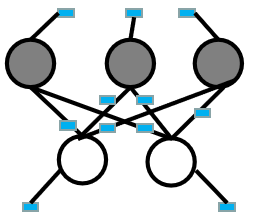
\includegraphics[width=.3\textwidth]{微信图片_20200229004607.png}
    \caption{受限玻尔兹曼机的因子图}
    \label{fig:my_label_1}
\end{figure}

我们可以看到因子的种类可以分成三种,可以分为一组边和两组点的因子。因子和点或者边进行组合就得到了公式(8)一样的形式。

\subsection{Restricted Boltzmann Machine概率密度函数}
所以Restricted Boltzmann Machine概率密度函数的表现形式如下所示:
\begin{equation}
    \begin{split}
    P(X) 
    = & \frac{1}{Z} \exp(h^T w v)\exp(\alpha^T v)\exp(\beta^T h) \\
    \end{split}
\end{equation}

而其中:
\begin{equation}
    \begin{split}
        \exp(h^T w v) =  \exp(\sum_{i=1}^m \sum_{j=1}^n h_iw_{ij}v_i) = \prod_{i=1}^m \prod_{j=1}^n \exp( h_iw_{ij}v_i) 
    \end{split}
\end{equation}

用类似的方法进行转换,我们可以得到:
\begin{equation}
    P(X) 
    = \frac{1}{Z} \underbrace{\prod_{i=1}^m \prod_{j=1}^n \exp( h_iw_{ij}v_i)}_{\mathrm{edge}} \underbrace{\prod_{j=1}^n \exp( \alpha_jv_j)}_{\mathrm{node}\ v} \underbrace{\prod_{i=1}^m \exp( \beta_ih_i)}_{\mathrm{node}\ h} 
\end{equation}

\subsection{小结}
本小节首先讲解了,为什么要有Restricted Boltzmann Machine?原因很简单,Boltzmann Machine的复杂度太高。大家有没有觉得Restricted Boltzmann Machine的结构很像神经网络,它和神经网络之间有什么不可告人的秘密呢?然后从点和边的角度对其进行了分解,然后得到了它的概率密度函数。下一节将RBM和之前的东西结合起来,因为它本质上还是一种无向图。

\section{RBM和其他概率图模型的联系}
RBM本质上还是一种无向图,所以我们把之前的东西都总结一下联系起来,来一起看看RBM的发展历史。

\subsection{Naive Bayes}
朴素贝叶斯算法是最简单的PGM,也是最基础的模型。此算法的核心就是朴素贝叶斯假设,或者说是条件独立假设。这个假设描述的是,当label $y$已知的情况下,各个属性之间是相互独立的。公式表达为:
$x_i\perp x_j|y$。朴素贝叶斯概率图如下所示:
\begin{figure}[H]
    \centering
    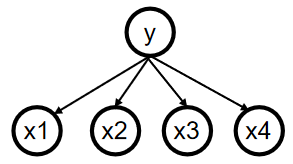
\includegraphics[width=.35\textwidth]{微信图片_20200229202910.png}
    \caption{朴素贝叶斯概率图模型}
    \label{fig:my_label_1}
\end{figure}

\subsection{Gaussian Mixture Model}
高斯混合模型中引入了隐变量,$y$是一个隐变量,$x$是观测变量。Gaussian Mixture Model概率图模型如下所示:
\begin{figure}[H]
    \centering
    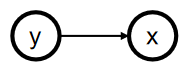
\includegraphics[width=.2\textwidth]{微信图片_20200229204430.png}
    \caption{高斯混合模型概率图模型}
    \label{fig:my_label_1}
\end{figure}
\noindent $y$是隐变量,并且是一个离散变量,一共有$k$种选择。并且在$y$给定的情况下,$x$符合一个高斯分布,即为:$P(x|y)\sim$Gaussian Distribution。在此模型中,$y$是一个离散的变量,如果将其扩充为一个变量序列(Sequence),就演变成了State Space Model。

\subsection{State Space Model}
State Space Model的主要特点就是两个:

1. 引入了隐变量,也就是State;

2. 符合两个假设,即为齐次马尔可夫假设和观测独立假设,这两个假设在之前都有过非常详细的介绍。

而State Space Model,大致可以分为三类:1. Hidden Markov Model;2. Kalman Filter;3. Particle Filter。

其中,Hidden Markov Model要求隐变量之间都是离散的;Kalman Filter是线性高斯系统,隐变量之间的转移概率和隐变量到观测变量之间,或者说是转移矩阵和发射矩阵之间都符合高斯分布;
Particle Filter是在Kalman Filter的基础上解除了线性高斯分布,认为转移矩阵和发射矩阵之间可以是很复杂的未知分布,通常采用采用的方法来近似求解。这三种模型的概率图模型都一样,如下图所示:
\begin{figure}[H]
    \centering
    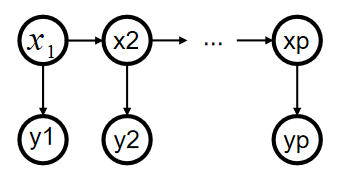
\includegraphics[width=.35\textwidth]{微信图片_20200229220207.png}
    \caption{State Space Model概率图模型}
    \label{fig:my_label_1}
\end{figure}

\subsection{Maximum Entropy Markov Model}
Logistics Regression是一种特殊的最大熵模型,简单的说就是最大熵模型求解出的分布是指数族分布。利用最大熵与HMM结合,就得到了MEMM。并且与HMM还有一点主要的不同就是
改变了$y$与$x$之间的有向图方向。MEMM概率图模型如下所示:
\begin{figure}[H]
    \centering
    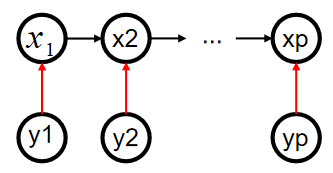
\includegraphics[width=.35\textwidth]{微信图片_20200229215807.png}
    \caption{Maximum Entropy Markov Model概率图模型}
    \label{fig:my_label_1}
\end{figure}
MEMM有两条主要的性质:1. 这是一个判别模型,MEMM主要解决的是标注问题,其中没有隐变量。2. 打破了观测独立假设。

\subsection{Conditional Random Field}
因为MEMM存在局部归一化的问题,为了解决这个问题,将$x$之间的有向图变成了无向图就得到了条件随机场。而同时也打破了齐次马尔可夫假设。同样CRF主要解决的是标注问题,其中没有隐变量,也是判别模型。概率图模型如下所示:
\begin{figure}[H]
    \centering
    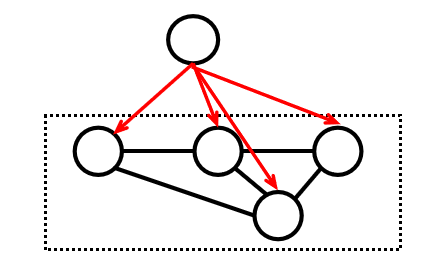
\includegraphics[width=.35\textwidth]{微信图片_20200229221504.png}
    \caption{Conditional Random Field概率图模型}
    \label{fig:my_label_1}
\end{figure}
但是,我们通常说的是Linear Chain Condition Random Field (LC-CRF),也就是马尔可夫随机场是线型的,概率图模型如下所示:
\begin{figure}[H]
    \centering
    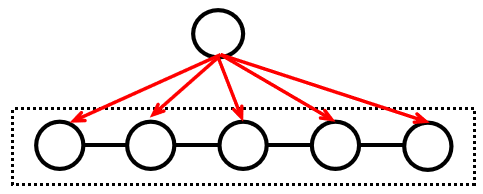
\includegraphics[width=.35\textwidth]{微信图片_20200229222221.png}
    \caption{Linear Chain Condition Random Field概率图模型}
    \label{fig:my_label_1}
\end{figure}
\subsection{Boltzmann Machine}
Boltzmann Machine本章节已经详细的描述过了,这里不再啰嗦了。主要三个特点:1. 无向图;2. 引入了隐变量;3. 所有节点的联合概率PDF必须是指数族分布,被称为Boltzmann Distribution或者是Gibbs Distribution。概率图模型如下所示:
\begin{figure}[H]
    \centering
    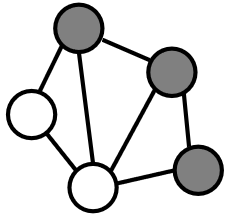
\includegraphics[width=.2\textwidth]{微信图片_20200228220817.png}
    \caption{Boltzmann Machine概率图模型}
    \label{fig:my_label_1}
\end{figure}

\subsection{Restricted Boltzmann Machine}
Boltzmann Machine的算法复杂度太高了,假设观测节点集合内部所有的节点之间相互独立,不可观测节点集合内部所有的节点之间相互独立,就得到了Restricted Boltzmann Machine。概率图如下所示:
\begin{figure}[H]
    \centering
    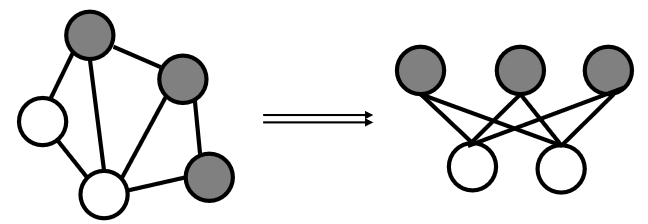
\includegraphics[width=.55\textwidth]{微信图片_20200229000824.png}
    \caption{Restricted Boltzmann Machine概率图模型}
    \label{fig:my_label_1}
\end{figure}

\subsection{小结}
概率图模型和条件独立之间有着不可划分的关系。条件独立性是尽可能的保留数据之间的结构信息,同时又简化计算。比如,朴素贝叶斯中的条件独立假设是在给定$y$的情况下,属性与属性之间是相互独立的。而State Space Model中的两个假设也是条件独立的。

概率图模型表示可以从以下五个方面分析:
\begin{itemize}
    \item 方向:(有向图/无向图)对应着Bayesian Network和Markov Random Field,很显然有向图有着更强的限制。\textbf{这是从边的角度进行分析。}
    \item 节点的变量是离散/连续:通常情况下,无特殊说明,都认为变量是离散变量。如果,变量是连续的,则为Gaussian Network。当然,也可以是混合的,部分为离散变量,部分为连续变量。\textbf{这是从点的角度进行分析。}
    \item 条件独立性:NB中的条件独立性是在随机变量各属性之间;HMM中就是齐次马尔可夫假设和观测独立假设上表示了条件独立性;MEMM打破了观测独立假设,仍然是在条件独立性上做文章;RBM的条件独立性表现在,给定观测变量的情况下,隐变量之间是条件独立的。当然,不仅属性之间可以是条件独立的,结构上也可以使条件独立的。\textbf{这是从边的角度进行分析。}
    \item 隐变量:是否引入隐变量也是一条重要的性质。Boltzmann Machine和马尔可夫随机场最重要的区别,就是Boltzmann Machine中将节点分成两类,可观测和不可观测。\textbf{这是从点的角度进行分析。}
    \item PDF是否是指数族分布:PDF是指节点的联合概率分布函数。根据最大熵原理,在给定数据的情况下,指数族分布是使得预测分布熵最大的分布。而BM的PDF一定是一个指数族分布。如果,图结构一个小局部,或者是指数族分布,在计算上也更加有优势。
\end{itemize}

\textbf{实际上,仔细回想,各种概率图模型说白了就是在这5个性质上进行组合,有或者没有,有的话强弱也可以不一样。概率图模型的表示,主要就是围绕这5点来做文章的。}

\section{The Inference of Restricted Boltzmann Machine}
前面我们已经详细的介绍过了Restricted Boltzmann Machine。假设一共有$p$个节点,其中$m$个不可观测的节点组成集合$h$,$n$个可观测的节点组成集合$v$。概率图模型如下所示:
\begin{figure}[H]
    \centering
    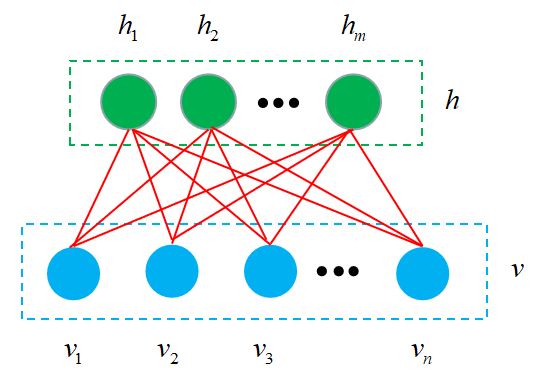
\includegraphics[width=.45\textwidth]{微信图片_20200229233931.png}
    \caption{Restricted Boltzmann Machine概率图模型}
    \label{fig:my_label_1}
\end{figure}
公式化表达如下所示,即为:
\begin{equation}
    X = \begin{bmatrix}
    x_1 \\
    x_2 \\
    \vdots \\
    x_p
    \end{bmatrix}
    = 
    \begin{bmatrix}
    h \\
    v
    \end{bmatrix}
    ,\quad
    h = 
    \begin{bmatrix}
    h_1 \\
    h_2\\
    \vdots \\
    h_m
    \end{bmatrix}
    ,\quad
    v = 
    \begin{bmatrix}
    v_1 \\
    v_2\\
    \vdots \\
    v_n
    \end{bmatrix}
\end{equation}
其中,$m+n=p$。节点的联合概率密度函数为:
\begin{equation}
    \begin{split}
        P(X) 
        =  \frac{1}{Z} \exp (-\mathrm{E}(X)) 
        \Longleftrightarrow P(v,h) 
        =   \frac{1}{Z} \exp (-\mathrm{E}(v,h)) \\
    \end{split}
\end{equation}
而其中,
\begin{equation}
\begin{split}
    \mathrm{E}(v,h) = & - h^T w v + \alpha^T v + \beta^T h \\
    = & - \left( \sum_{i=1}^m \sum_{j=1}^n h_iw_{ij}v_i + \sum_{j=1}^n \alpha_j v_j + \sum_{i=1}^m \beta_i h_i 
    \right)
\end{split}
\end{equation}

\textbf{个人觉得机器学习中,研究问题的主要流程基本可以拆解成,首先1. 需要知道模型怎么表示(Representation);2. 然后,通过数据的学习来得到模型的参数(Learning);3. 最后,利用模型来对未知的数据进行推断(Inference)。}

\subsection{明确Inference的问题}
\noindent 首先假设Learning的过程已经完成,那么所有的参数我们都已经知道了,所以我们已知的有:
{\color{red}

1. 所有的势函数,这样归一化因子就知道了;

2. 能量函数;

3. 知道能量函数就知道$h$和$v$的联合概率分布$P(v,h)$。
}

~\\

\noindent 需要Inference的是三个问题:

1. $P(h|v)$;

2. $P(v|h)$;

3. $P(v)$。

然而,为什么不求$P(v)$呢?实际上求$P(h)$的边缘概率没什么必要,我们更多的是关注在已知$v$的情况下,$P(h|v)$的条件概率分布。$P(h)$中$h$反正也是不可观测的,求了边缘概率分布也没什么用。如果要求解的话和求解$P(v)$的方法一样。

\subsubsection{求解$P(h|v)$ and $P(v|h)$}
$P(h|v)$和$P(v|h)$求解方法都是一样的,这里就放在一起推导。

$P(h|v)$求解的是$v$中所有节点都知道的情况下,集合$h$的联合概率分布,即为:
$$
P(h_1,h_2,\cdots,h_m|v)
$$

那么,首先我们就要根据条件独立性来对联合概率分布进行化简。那么,我们想想$h_i\perp h_j|v,\ i\neq j$是成立的吗?其实一看就知道是成立的。为什么呢?无向图满足局部马尔可夫性质,这个性质的意思是,当无向图中一个节点,除这个节点以外的所有节点都知道的话,这个节点只和他的邻居有关,和其他节点都是独立的。也就是\textbf{{\color{red}$P(h_i|-h_i,v) = P(h_i|$邻居节点$)=P(h_i|v)$}}。根据:
$$
P(h_i|-h_i,v) =P(h_i|v)
$$
我们就可以得到$h_i\perp h_j|v,\ i\neq j$。所以,根据条件独立性,联合概率(联合后验概率)可以被简化为:
\begin{equation}
    P(h|v) = \prod_{l=1}^m P(h_l|v)
\end{equation}
为了简化,我们假设无向图所有节点都是二值的,也就是$h,v\in \{0,1 \}$。实际上RBM的节点是离散变量,而0/1分布是最简单的离散分布。但是,为了详细的解析,这里用了简单的分布来进行解析,其他的离散分布形式可以看成是0/1分布的变种。

那么,假设我们要求的是$P(h_l=1|v)$,我们已经知道的是$P(v,h)$。那么自然就想到将$h$补齐,我们用$h_{-l}$来表示除$h_l$外的所有节点,所以有:
\begin{equation*}
    \begin{split}
        P(h_l=1|v) = & P(h_l=1|h_{-l},v) = \frac{P(h_l=1,h_{-l},v)}{P(h_{-l},v)} = \frac{P(h_l=1,h_{-l},v)}{\sum_{h_l} P(h_l,h_{-l},v)} \\
        = & \frac{P(h_l=1,h_{-l},v)}{P(h_l=1,h_{-l},v)+P(h_l=0,h_{-l},v)}
    \end{split}
\end{equation*}

~\\

那么,怎么求解呢?首先看分子怎么求。$P(h_l=1,h_{-l},v)$非常的特殊,和联合概率分布不一样的地方在于其中某一个变量的状态是已知的。那么我们把这个变量从联合概率中分解出来,赋予具体的值就可以了。

于是,我们的下一步操作就是对能量函数进行改写,将$h_l$相关的项解析出来。实际上就是和$h_l$自己和相关的边有关。
\begin{equation}
\begin{split}
    \mathrm{E}(v,h)= & - \left( \sum_{i=1}^m \sum_{j=1}^n h_iw_{ij}v_i + \sum_{j=1}^n \alpha_j v_j + \sum_{i=1}^m \beta_i h_i \right)  \\
    = & \left( \underbrace{\sum_{i=1,i\neq l}^m \sum_{j=1}^n h_iw_{ij}v_i}_{\triangle_1} + \underbrace{\sum_{j=1}^n h_lw_{lj}v_i}_{\triangle_2} + \underbrace{\sum_{j=1}^n \alpha_j v_j}_{\triangle_3} + \underbrace{\sum_{i=1,i\neq l}^m \beta_i h_i}_{\triangle_4} +\underbrace{ \beta_l h_l }_{\triangle_5} \right)  
\end{split}
\end{equation}

令$H_l(v)=\triangle_2+\triangle_5$,表示和$h_l$相关的部分,很显然因为$h_l$已知,不含和$h$相关的部分了;

令$\Bar{H}_l(h_{-l},v)=\triangle_1+\triangle_3+\triangle_4$,表示和$h_l$不相关的部分;所以:
\begin{equation*}
    \begin{split}
        H_l(v)=\triangle_2+\triangle_5 = h_l\left( \sum_{j=1}^n w_{lj}v_i + \beta_l \right)
    \end{split}
\end{equation*}
我们将$\sum_{j=1}^n w_{lj}v_i + \beta_l$定义为$ H_l(v)$,所以:
\begin{equation}
    \mathrm{E}(v,h) = h_lH_l(v) + \Bar{H}_l(h_{-l},v)
\end{equation}
那么,分子为:
\begin{equation}
    P(h_l=1,h_{-l},v) = \frac{1}{Z}\exp\left\{ h_l(v) + \Bar{H}_l(h_{-l},v) \right\}
\end{equation}
那么,分母为:
\begin{equation}
    P(h_l=1,h_{-l},v) + P(h_l=0,h_{-l},v) = \frac{1}{Z}\exp\left\{ h_l(v) + \Bar{H}_l(h_{-l},v) \right\} + \frac{1}{Z}\exp\left\{ \Bar{H}_l(h_{-l},v) \right\}
\end{equation}
所以,
\begin{equation}
\begin{split}
    P(h_l=1|v) = & \frac{P(h_l=1,h_{-l},v)}{P(h_l=1,h_{-l},v) + P(h_l=0,h_{-l},v)} \\
    = & \frac{\frac{1}{Z}\exp\left\{ h_l(v) + \Bar{H}_l(h_{-l},v) \right\}}{\frac{1}{Z}\exp\left\{ h_l(v) + \Bar{H}_l(h_{-l},v) \right\} + \frac{1}{Z}\exp\left\{ \Bar{H}_l(h_{-l},v) \right\}} \\
    = & \frac{1}{1+\exp\left\{ \Bar{H}_l(h_{-l},v) - h_l(v) - \Bar{H}_l(h_{-l},v) \right\}} \\
    = & \frac{1}{1+\exp\left\{ - h_l(v) \right\}}
\end{split}
\end{equation}
而$\frac{1}{1+\exp\left\{- h_l(v)\right\}}$实际就是Sigmoid函数,Sigmoid函数的表达形式为:$\sigma(x) = \frac{1}{1+e^{-x}}$。
\begin{equation}
    P(h_l=1|v) = \sigma( h_l(v)) = \sigma(\sum_{j=1}^n w_{lj}v_i + \beta_l)
\end{equation}

既然已经求得了$P(h_l|v)$,根据公式(15)就可以得到$P(h|v)$的结果了:
\begin{equation}
    P(h|v) = \prod_{l=1}^m P(h_l|v) = \left( \sigma\left(\sum_{j=1}^n w_{lj}v_i + \beta_l\right) \right)^k\left(1-\sigma\left(\sum_{j=1}^n w_{lj}v_i + \beta_l\right)\right)^{m-k}
\end{equation}
其中$k$为$h$集合中,$h_l=1$的节点数。

~\\

已经成功求得了$P(h|v)$,那么求解$P(v|h)$的过程是一模一样的,基本上可以做一个转换,直接得到结果:
\begin{equation}
    P(v|h) = \prod_{l=1}^m P(h_l|v) = \left( \sigma\left(\sum_{j=1}^m w_{jl}h_j + \alpha_l\right) \right)^k\left(1-\sigma\left(\sum_{j=1}^m w_{jl}h_j + \alpha_l\right)\right)^{n-k}
\end{equation}
其中$k$为$v$集合中,$v_l=1$的节点数。

那么,到这里对于后验的计算已经完成了,后验实际上就是Sigmoid函数。大家有没有觉得RBM和神经网络很像,我其实早就有这种感觉了,不可观测节点不就是隐藏层。而Sigmoid函数,经常被用来当做神经网络的激活函数。这之间是巧合还是有必然的联系呢?后面的章节我们会有分析的,神经网络实际上是从RBM中发展得到的。

\subsection{求解$P(v)$(inference$\rightarrow$ marginal $\rightarrow$ $P_{v}$)}
这一小节,我们的目标是通过Inference来求解Marginal Distribution $P(v)$。思路很简单,既然我们知道联合概率分布$P(v,h)$,那么把$h$节点的变量积分掉不就可以了,所以:
\begin{equation}
\begin{split}
    P(v) = & \sum_h P(v,h) = \sum_h \frac{1}{Z} \exp \left\{ -\mathrm{E}(v,h) \right\} = \frac{1}{Z} \sum_h  \exp (h^T w v + \alpha^T v + \beta^T h ) \\
    = & \frac{1}{Z} \sum_{h_1}\cdots \sum_{h_m} \exp (h^T w v + \alpha^T v + \beta^T h )\\
    = & \frac{1}{Z} \exp(\alpha^T v) \sum_{h_1}\cdots \sum_{h_m} \exp (h^T w v + \beta^T h )\\
\end{split}
\end{equation}

我们下一步的目标就是将等式(24)中的所有和$h$相关的项提取出来,分别进行计算。为了方便计算,我们令:
\begin{equation}
    h = 
   \begin{bmatrix}
    h_1 \\
    h_2\\
    \vdots \\ 
    h_m
    \end{bmatrix}, \ h_l\in\{0,1\}\qquad
    w=[w_{ij}]_{m\times n} = 
    \begin{bmatrix}
    ---w_1^{T}---\\
    ---w_2^{T}---\\
    \vdots \\
    ---w_m^{T}---\\
    \end{bmatrix}
\end{equation}
这里的$w$,我们用$m$个行向量来表示。那么,
$$
h^T w v = \begin{bmatrix}
    h_1 & h_2 & \cdots & h_m
    \end{bmatrix}
    \begin{bmatrix}
    ---w_1^{T}---\\
    ---w_2^{T}---\\
    \vdots \\
    ---w_m^{T}---\\
    \end{bmatrix}v = \sum_{i=1}^m h_iw_i^{T}v
$$
$$
\beta^Th = \sum_{i=1}^m \beta_i h_i
$$
所以,
\begin{equation}
    \begin{split}
        P(v) = & \frac{1}{Z} \exp(\alpha^T v) \sum_{h_1}\cdots \sum_{h_m} \exp \left(\sum_{i=1}^m h_iw_i^{T}v + \sum_{i=1}^m \beta_i h_i\right)\\
        = & \frac{1}{Z} \exp(\alpha^T v) \sum_{h_1}\cdots \sum_{h_m} \exp \left(\sum_{i=1}^m (h_iw_i^{T}v + \beta_i h_i)\right)\\
        = & \frac{1}{Z} \exp(\alpha^T v) \sum_{h_1}\cdots \sum_{h_m} \exp \left(\sum_{i=1}^m (h_iw_i^{T}v + \beta_i h_i)\right)\\
        = & \frac{1}{Z} \exp(\alpha^T v) \sum_{h_1}\cdots \sum_{h_m} \exp \left((h_1w_1^{T}v + \beta_1 h_1)+(h_2w_2^{T}v + \beta_2 h_2)\cdots (h_mw_m^{T}v + \beta_m h_m)\right)\\
        = & \frac{1}{Z} \exp(\alpha^T v) \sum_{h_1}\exp (h_1w_1^{T}v + \beta_1 h_1) \sum_{h_2}(h_2w_2^{T}v + \beta_2 h_2) \cdots \sum_{h_m}(h_mw_m^{T}v + \beta_m h_m)
    \end{split}
\end{equation}
由于$h_l \in\{0,1\}$,所以,
\begin{equation}
\begin{split}
    P(v) = &\frac{1}{Z} \exp(\alpha^T v) \sum_{h_1}\exp (h_1w_1^{T}v + \beta_1 h_1) \sum_{h_2}(h_2w_2^{T}v + \beta_2 h_2) \cdots \sum_{h_m}(h_mw_m^{T}v + \beta_m h_m) \\
    = &\frac{1}{Z} \exp(\alpha^T v) \left[ 1+\exp(w_1v+\beta_1) \right]\cdots \left[ 1+\exp(w_m^{T}v+\beta_m) \right] \\
    = & \frac{1}{Z} \exp(\alpha^T v) \exp \left[\log ( 1+\exp(w_1^{T}v+\beta_1)) \right]\cdots \exp \left[\log ( 1+\exp(w_m^{T}v+\beta_m)) \right] \\
    = & \frac{1}{Z} \exp\left(\alpha^T v + \sum_{i=1}^m \log ( 1+\exp(w_i^{T}v+\beta_i)) \right)
\end{split}
\end{equation}

而$\log ( 1+\exp(w_i^{T}v+\beta_i))$是一种softplus函数的形式,softplus函数可以描述为:$\mathrm{softplus}(x) = \log(1+e^x)$,函数图像如下所示:
\begin{figure}[H]
    \centering
    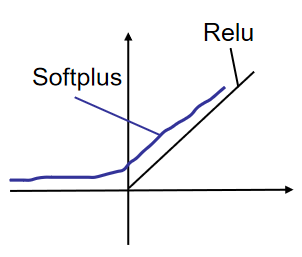
\includegraphics[width=.45\textwidth]{微信图片_20200301132709.png}
    \caption{Softplus函数图像}
\end{figure}
我们可以看到此函数在正半轴越来越接近Relu函数,所以,接着公式(27)继续向下推导得:
\begin{equation}
\begin{split}
    P(v) = & \frac{1}{Z} \exp\left(\alpha^T v + \sum_{i=1}^m \log ( 1+\exp(w_iv+\beta_i)) \right) \\
    = &\frac{1}{Z} \exp\left(\alpha^T v + \sum_{i=1}^m \mathrm{softplus} ( w_iv+\beta_i) \right)
\end{split}
\end{equation}
那么,就可以求得关于$v$的边缘概率分布了。$v$可能有$k$种状态,将每种状态的具体值代入即可。最后在总结一下:
\begin{equation}
    P(v)
    = \frac{1}{Z} \exp\left(\alpha^T v + \sum_{i=1}^m \mathrm{softplus} ( w_iv+\beta_i) \right)
\end{equation}
其中,$w_i$为$w$矩阵的行向量。
\subsection{小结}
在本小节中,我们主要计算了三个推断问题,$P(v|h)$,$P(h|v)$,$P(v)$。计算结果如下所示:
\begin{equation}
    \begin{split}
    & P(v|h) = \prod_{l=1}^m P(h_l|v) = \left( \sigma\left(\sum_{j=1}^m w_{jl}h_j + \alpha_l\right) \right)^k\left(1-\sigma\left(\sum_{j=1}^m w_{jl}h_j + \alpha_l\right)\right)^{n-k} \\
    & P(h|v) = \prod_{l=1}^m P(h_l|v) = \left( \sigma\left(\sum_{j=1}^n w_{lj}v_i + \beta_l\right) \right)^k\left(1-\sigma\left(\sum_{j=1}^n w_{lj}v_i + \beta_l\right)\right)^{m-k} \\
    & P(v)
    =  \frac{1}{Z} \exp\left(\alpha^T v + \sum_{i=1}^m \mathrm{softplus} ( w_iv+\beta_i) \right) \\
    \end{split}
\end{equation}

我看计算的思路都差不多,都是把已知条件分类出来,然后赋予具体的值。我们采用的离散分布是0/1分布是为了简化计算,当值具有多个时,计算的思路也是一样的。\textbf{但是,无论可能的取值变成多少个,整体还是符合指数族分布的。}

\section{Conclusion}
本章节,主要描述了Restricted Boltzmann Machine。主要的讲述思路是先从马尔可夫随机场中引出了Boltzmann Machine,介绍了什么是Boltzmann Machine;然后描述了Boltzmann Machine的计算intractable,然后引出了Restricted Boltzmann Machine;紧接着介绍了Restricted Boltzmann Machine模型表示方法,并讲述了它在概率图模型整体结构中的地位;最后讲述了如何用Restricted Boltzmann Machine来进行推断。

大家可能发现,在使用模型Inference的时候,需要通过Learning来从数据中得到参数的值,这部分会在之后的直面配分函数中描述。












\end{document}